% ---------
%  Compile with "pdflatex hw0".
% --------
%!TEX TS-program = pdflatex
%!TEX encoding = UTF-8 Unicode

\documentclass[11pt]{article}
\usepackage{jeffe,handout,graphicx}
\usepackage[utf8]{inputenc}		% Allow some non-ASCII Unicode in source

% =========================================================
%   Define common stuff for solution headers
% =========================================================
\Class{CS/ECE 374 A}
\Semester{Spring 2018}
\Authors{3}
\AuthorOne{Violet Baudelaire}{vbeaudel}
\AuthorTwo{Friday Caliban}{fcaliban}
\AuthorThree{Duncan Quagmire}{dquagmir}
%\Section{}

% =========================================================
\begin{document}

% ---------------------------------------------------------


\HomeworkHeader{0}{2}	% homework number, problem number

\begin{solution}
These are, without exception, inappropriate inquiries, a phrase which here means “all the wrong questions”.  Here are the questions you should have asked instead:
\begin{enumerate}[(a)]
\item Why would someone say something was stolen when it was never theirs to begin with?
\item How could someone who was missing be in two places at once?
\item Why would someone destroy one building when they really wanted to destroy another?
\end{enumerate}
\end{solution}

\begin{solution}[for 25\%]
Pietrisycamollaviadelrechiotemexity!
\end{solution}

% ---------------------------------------------------------
% Change authors for all future solutions
\AuthorOne{Marceline Abadeer}{mabadeer}
\AuthorTwo{Finn Mertens}{fmertens}
\AuthorThree{Simon Petrikov}{iceking@ooo.org}
\HomeworkHeader{0}{1}

\newtheorem{lemma}{Lemma}

\begin{solution}[R. Rotten]
Alright! I can see that I will have to teach you how to be \emph{villains!}

\begin{enumerate}[(a)]
\item
Now listen closely.  Here's a little lesson in trickery.  This is going down in history.
If you wanna be a Villain Number One, you have to chase a superhero on the run.  Just follow my moves, and $^{\emph{sneak}}$ around.  Be careful not to make a sound!
Shh!  No, don't touch that!

\[
	We = \#1^\text{Hey!}
\]

\item~
\begin{algo}
	\textul{\textsc{HaHaHa}(\emph{net}):}\+
\\	$\emph{net}.\emph{found} \gets \emph{now}$
\\	$\textsc{LookAt}(\emph{net})$
\\	in parallel:\+
\\		for $i\gets 1$ to $100$\+
\\			if $\emph{said\_go} = \textsc{True}$\+
\\				$\emph{net}.\emph{ReadyToThrow} \gets \textsc{True}$\-\-
\\		$\emph{said\_go} \gets \textsc{True}$\-
\\[0.5ex]
	if \emph{net}.\emph{ReadyToThrow}\+
\\		$\textsc{Throw}(\emph{net}, \emph{him}, \lnot me)$\-
\\	\textsc{Try}(\emph{banana}.\emph{peel})
\end{algo}

\begin{algo}
	\textul{$\textsc{Try}(\emph{somethingelse})$:}\+
\\	$\textsc{Watch}(\,)$
\\	$\textsc{Learn}(\,)$
\\	$\emph{deal}.\emph{location} \gets \emph{here}$
\\	return $\textsc{Slip}(\emph{somethingelse}) \land
				\textsc{Slide}(\emph{somethingelse})$
\end{algo}

$\textsc{HaHaHa}(\emph{Gasp!})$   What are you \emph{doing!?}

\item
Ba-ba-biddly-ba-ba-ba-ba,\footnote{According to \url{https://genius.com/Lazy-town-we-are-number-one-lyrics}.  It sounds more like “Daah-dat-dadyadyat-dat-dah-dah\dots” to me, but whatever.} ba-ba-ba-ba-ba-ba-ba, we are number one. Hey!\\
Ba-ba-biddly-ba-ba-ba-ba, ba-ba-ba-ba-ba-ba-ba, \textbf{VILLAIN NUMBER ONE!}\footnote{Genius Lyrics missed this line entirely.}

\item
Ba-ba-biddly-ba-ba-ba-ba, ba-ba-ba-ba-ba-ba-ba, we are number one. Hey!\\
Ba-ba-biddly-ba-ba-ba-ba, ba-ba-ba-ba-ba-ba-ba, we are number one. Hey!\\
We are number one, hey!  We are number one!  We are number one!  Hey! Hey!
\end{enumerate}
\end{solution}

% ---------------------------------------------------------
% Change authors again ; you can omit this if the authors aren’t changing.
\AuthorOne{Hunson Abadeer}{habadeer}
\AuthorTwo{Martin Mertens}{mmertens}
\AuthorThree{Urgence Evergreen}{gunterno}

\HomeworkHeader{0}{3}


\begin{solution}
Let $n$ be an arbitrary non-negative integer. There are four cases to consider:
\begin{itemize}
\item
Makin’ pancakes, makin’ bacon pancakes

\item
Make some bacon and I put it in a pancake

\item
\reflectbox{\raisebox{-0.5\height}{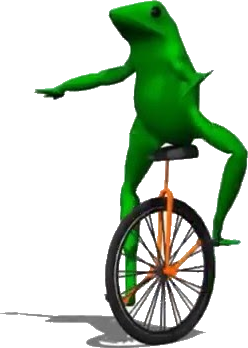
\includegraphics[scale=0.2]{Fig/datboi}}}
\raisebox{-0.5\height}{
\includegraphics[scale=0.4]{Fig/pancakes2}}
\raisebox{-0.5\height}{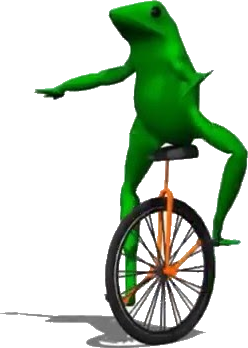
\includegraphics[scale=0.2]{Fig/datboi}}

\item
O shit waddup
\end{itemize}
\end{solution}



\end{document}
